\question \textbf{Bellman-Ford}

Use the Bellman-Ford algorithm (see lecture script) to determine the shortest path from source z to any other node in the graph.

\begin{solution}
    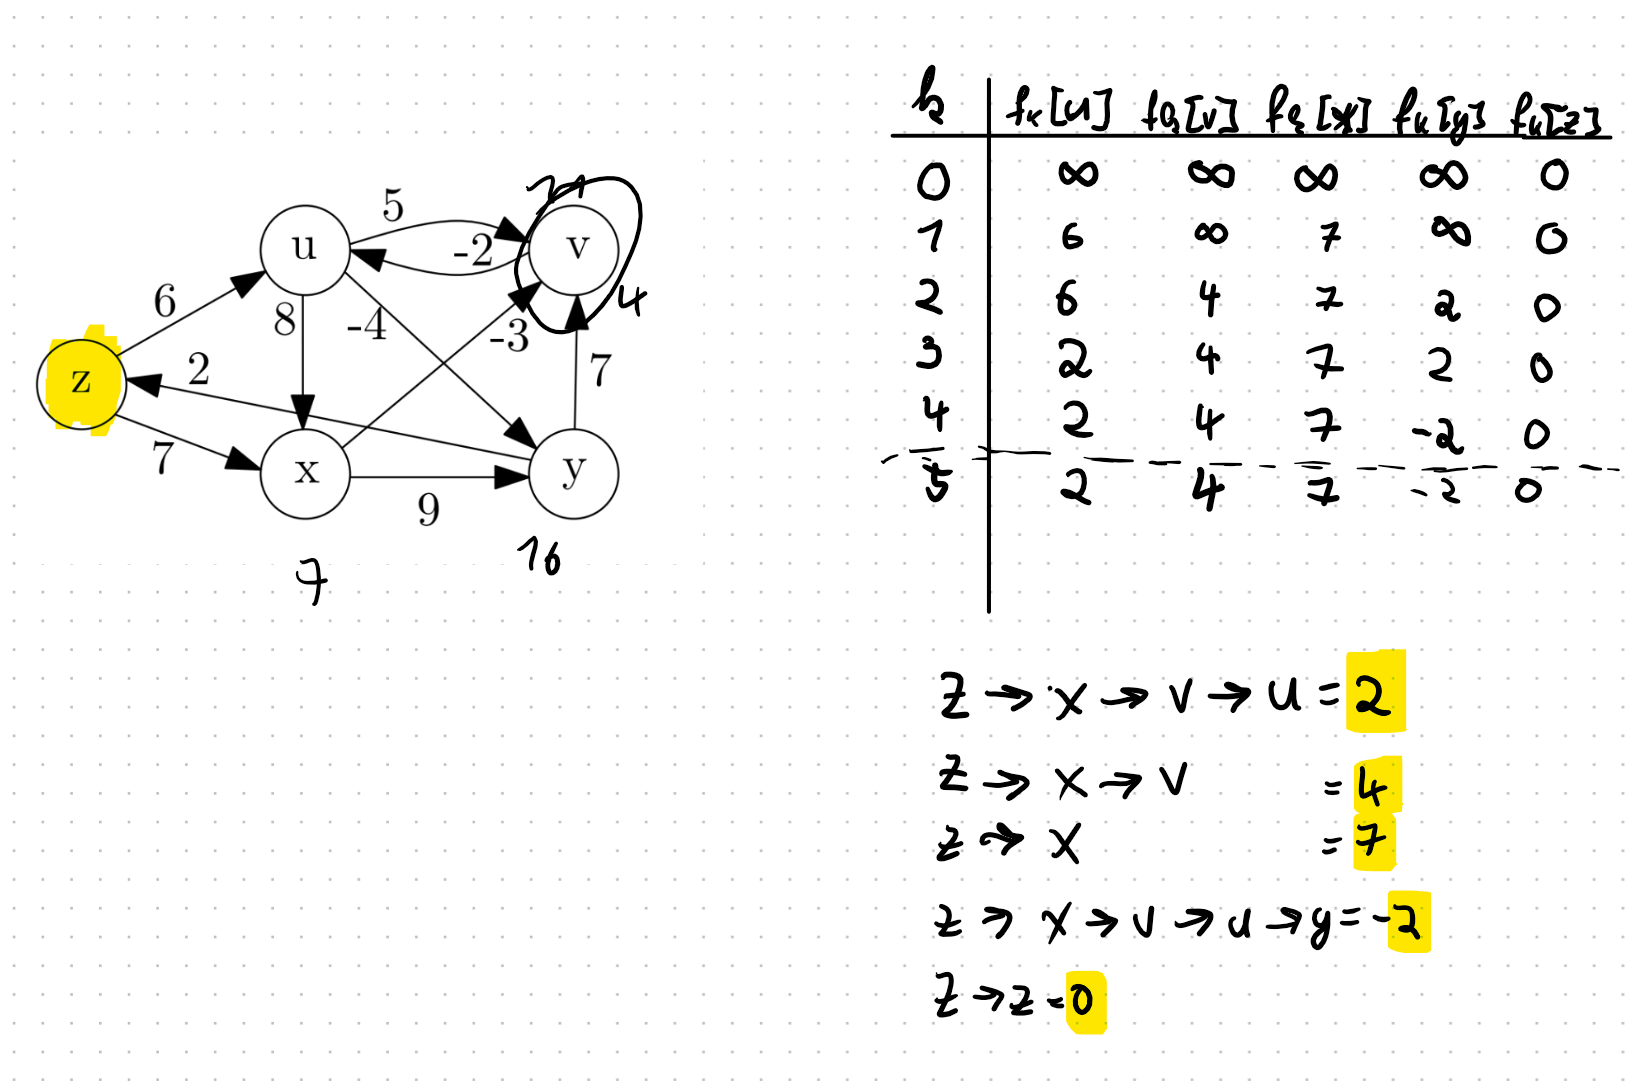
\includegraphics[width=0.8\linewidth]{task_2/sheet09_a2.png}
    
\end{solution}


% For tasks without simply remove the \begin{parts}...\part...\end{parts} commands